\documentclass[12pt]{article}
\usepackage{float}
\usepackage[dvipsnames]{xcolor}
\usepackage{dingbat, tikz}
\usepackage{amsfonts,amsmath, color, graphicx, mathtools, empheq, amsthm, amssymb}
\usepackage{wasysym}
\usepackage{thmtools}
\usepackage{listings}
\usepackage[framed]{mcode} % for matlab to be colored
%\usepackage{blindtext} % for sections
\usepackage{titlesec} % for custom sections

% custumoize margins
\addtolength{\oddsidemargin}{-.5in}
\addtolength{\evensidemargin}{-.5in}
\addtolength{\textwidth}{1.0in}

\addtolength{\topmargin}{-.875in}
\addtolength{\textheight}{1.75in}

% customize chapter/section formatting
\newcommand{\sectionfont}{\Large\bfseries}

\titleformat{\section}
    {\titlerule     
     \vspace{2.0ex}
     \normalfont}
    {\thesection}{1em}
    {\sectionfont}[\vspace{2.0ex}\titlerule]
\setcounter{secnumdepth}{0} % so sections arent numbered but can still make table of contents

% change table of contents title
\renewcommand*\contentsname{Table of Contents}


% to make fancy header on top of each page
\usepackage{fancyhdr}
\pagestyle{fancy}
\fancyhf{}
\rhead{Math 226B: Homework \#5}
\lhead{Gorman, Kara}
%\rfoot{Page \thepage}



\newtheorem{problem}{Problem}
\newtheorem{lemma}{Lemma}

% to put colored box around theorem\problem\lemma etc
\usepackage{tcolorbox}
% make custom box so I can specify the color
\newtcolorbox{mybox}[3][]
{
  colframe = #2!50!black,
  colback  = #2!10,
  coltitle = #2!20!black,  
  title    = #3,
  #1,
}


%To allow for matrix larger than 10x10
\setcounter{MaxMatrixCols}{11}

%To set thumbs up as QED symbol
\renewcommand{\qedsymbol}{\begingroup \color{blue} \rightthumbsup \endgroup}

%To make a new command for an asterisk in a circle
\newcommand{\circlesign}[1]{ 
    \mathbin{
        \mathchoice
        {\buildcirclesign{\displaystyle}{#1}}
        {\buildcirclesign{\textstyle}{#1}}
        {\buildcirclesign{\scriptstyle}{#1}}
        {\buildcirclesign{\scriptscriptstyle}{#1}}
    } 
}
\newcommand\buildcirclesign[2]{%
    \begin{tikzpicture}[baseline=(X.base), inner sep=0, outer sep=0]
    \node[draw,circle] (X)  {\ensuremath{#1 #2}};
    \end{tikzpicture}%
}

%To use a border matrix with brackets
\usepackage{etoolbox}
\let\bbordermatrix\bordermatrix
\patchcmd{\bbordermatrix}{8.75}{4.75}{}{}
\patchcmd{\bbordermatrix}{\left(}{\left[}{}{}
\patchcmd{\bbordermatrix}{\right)}{\right]}{}{}

%To make text in an equation smaller
\newcommand*{\Scale}[2][4]{\scalebox{#1}{$#2$}}
%\[\Scale[0.5]{y = \sin^2 x}\] %example of how ot use above command



\def\C{\mathbb{C}}
\def\N{\mathbb{N}}
\def\Q{\mathbb{Q}}
\def\R{\mathbb{R}}
\def\Ts{\mathbb{T}}
\def\Z{\mathbb{Z}}
\def\T{\mathcal{T}}
\def\P{\mathcal{P}}
\title{\underline{Math 226B: Homework \#5}}
\author{\huge Kara Gorman}
\begin{document}

%\begin{mybox}{blue}{}
%\begin{mybox}{Cerulean}{}
\maketitle
%\text{ }
%\end{mybox}
%\text{ }
%\end{mybox}
\bigskip\bigskip\bigskip\bigskip\bigskip\bigskip\bigskip\bigskip\bigskip\bigskip

\tableofcontents
\newpage


\section{Problem 1} \begin{mybox}{Cerulean}{}
Consider the following generalization of the two-dimensional problem on the unit square:
\begin{align}
-u_{xx} - u_{yy} + \gamma u_x &= f(x,y), \text{ } (x,y) \in R:=(0,1)\times (0,1),  \\
u &= g(x,y), \text{ } (x,y) \in \partial R.\nonumber
\end{align}
Here $\gamma >0$ is a parameter.\\
We discretize using the grid points
$$(x_j,y_k):=(jh,kh), \text{ } j,k=0,1,\dots,m+1,$$
where $m \geq 1$ is an integer and $h:=\frac{1}{m+1}$.  We employ centered differences to approximate $u_{xx}$ and $u_{yy}$ and the approximation
$$u_x \big\vert_{x=x_j, y=y_k} \approx \frac{u(x_{j+1},y_k) - u(x_{j-1},y_k)}{2h}$$
for $u_x$.  The resulting linear system is of the form
$$Av = b, \text{ } A = A_0 + \gamma A_1,$$
where $A_0$ is a symmetric positive definite matrix corresponding to the discretization of $-u_{xx} - u_{yy}$ and $A_1$ is a skew-symmetric matrix corresponding to the discretization of $u_x$.  Note that the matrix $A$ is nonsymmetric if $\gamma \neq 0$.\\
Use Matlab's "gmres" function with left preconditioning
$$M = A_0 = M_1 M_2, \text{ where } M_1=A_0 \text{ and } M_2=I,$$
to solve the linear system.  Employ your FFT-based algorithm from Problem 1 of Homework 3 for the solution of the linear systems with $M_1$.  This can be done by calling Matlab's GMRES routine with a function handle of a function that returns $A'v$, where
$$A' = M_1^{-1}A = I + \gamma M_1^{-1}A_1.$$
To test your Matlab program, solve problem (1) with the functions
$$f(x,y) = x^3y^2e^{2-x-y} \text{ and } g(x,y) = 1$$
for each of the parameter values
$$\gamma = 1, 10, 50, 100, 100.$$
In each case, choose $m=100$ for the discretization and run GMRES (without restarts) with zero initial guess $v_0 = 0$ and convergence tolerance tol = $10^{-10}$.\\
Print out the number of GMRES iterations and the relative residual norm RELRES of the final GMRES iterate.\\
How do your iteration counts depend on $\gamma$?
\end{mybox}

The centered difference approximation of (1) is:
%\begin{small}
\begin{align*}
\frac{1}{h^2}\bigg(4u_{j,k} - u_{j-1,k} - u_{j+1,k} - u_{j,k-1} - u_{j,k+1}\bigg) +\gamma\frac{1}{2h}\bigg(u_{j+1,k} - u_{j-1,k}\bigg) &= f \\
\bigg(4u_{j,k} - u_{j-1,k} - u_{j+1,k} - u_{j,k-1} - u_{j,k+1}\bigg) + \gamma\frac{h}{2}\bigg(u_{j+1,k} - u_{j-1,k}\bigg) &= h^2f \\
\bigg(T_mU + UT_m\bigg) + \gamma\frac{h}{2}\bigg(S_mU + US_m\bigg) &= h^2f \\
\begin{bmatrix}
T_m + 2I & -I & 0 & \hdots & 0 \\
-I & T_m + 2I & -I &  & \vdots\\
0 & -I & \ddots & \ddots & 0\\
\vdots &  & \ddots & & -I \\
0 & \hdots & 0 & -I & T_m + 2I \\
\end{bmatrix}U + \gamma\frac{h}{2}\begin{bmatrix}
0 & I & 0 & \hdots & 0 \\
-I & 0 & I &  & \vdots\\
0 & -I & \ddots & \ddots & 0\\
\vdots &  & \ddots & & I \\
0 & \hdots & 0 & -I & 0 \\
\end{bmatrix}U & = h^2f \\
\begin{bmatrix}
4 & -1 & 0 & \hdots & 0 \\
-1 & 4 & -1 &  & \vdots\\
0 & -1 & \ddots & \ddots & 0\\
\vdots &  & \ddots & & -1 \\
0 & \hdots & 0 & -1 & 4 \\
\end{bmatrix}U + \gamma\frac{h}{2}\begin{bmatrix}
0 & 1 & 0 & \hdots & 0 \\
-1 & 0 & 1 &  & \vdots\\
0 & -1 & \ddots & \ddots & 0\\
\vdots &  & \ddots & & 1 \\
0 & \hdots & 0 & -1 & 0 \\
\end{bmatrix}U & = h^2f
\end{align*}
%\end{small}
where $U = [u_{11} u_{21} \dots u_{mm}]^T$, $f = [f_{11} f_{21} \dots f_{mm}]^T$.\\
Now, to solve $Av = b$, we see that:
\begin{align*}
Av &= b \\
(A_0 + \gamma A_1)v &= f \\
A_0v + \gamma A_1v &= f \\
\frac{1}{h^2}\begin{bmatrix}
4 & -1 & 0 & \hdots & 0 \\
-1 & 4 & -1 &  & \vdots\\
0 & -1 & \ddots & \ddots & 0\\
\vdots &  & \ddots & & -1 \\
0 & \hdots & 0 & -1 & 4 \\
\end{bmatrix}v + \gamma \frac{1}{2h}\begin{bmatrix}
0 & 1 & 0 & \hdots & 0 \\
-1 & 0 & 1 &  & \vdots\\
0 & -1 & \ddots & \ddots & 0\\
\vdots &  & \ddots & & 1 \\
0 & \hdots & 0 & -1 & 0 \\
\end{bmatrix}v &= f \\
\begin{bmatrix}
4 & -1 & 0 & \hdots & 0 \\
-1 & 4 & -1 &  & \vdots\\
0 & -1 & \ddots & \ddots & 0\\
\vdots &  & \ddots & & -1 \\
0 & \hdots & 0 & -1 & 4 \\
\end{bmatrix}v + \gamma \frac{h}{2}\begin{bmatrix}
0 & 1 & 0 & \hdots & 0 \\
-1 & 0 & 1 &  & \vdots\\
0 & -1 & \ddots & \ddots & 0\\
\vdots &  & \ddots & & 1 \\
0 & \hdots & 0 & -1 & 0 \\
\end{bmatrix}v &= h^2f 
\end{align*}
So, we can set $b = fh^2$.\\
Next, we impose the boundary conditions on $f$ as follows, given that $ u = g(x,y) = 1$ for $(x,y) \in \partial R$:
\begin{align*}
b(1,:) &= b(1,:) + b_0 \\
b(m,:) &= b(m,:) + b_1 \\
b(:,1) &= b(:,1) + \gamma\frac{h}{2}c_0 + c_0 \\
b(:,m) &= b(:,m) - \gamma\frac{h}{2}c_1 + c_1 
\end{align*}
where $b_0, b_1, c_0, c_1$ are all vectors of ones, with length $m$.\\
Now, given our preconditioners $M1 = A_0$ and $M_2 = I$, then 
\begin{align*}
A' &= M_1^{-1}A \\
&= M_1^{-1}\big(A_0 + \gamma A_1\big) \\
&= A_0^{-1}A_0 + \gamma A_0^{-1}A_1 \\
&= I + \gamma A_0^{-1}A_1
\end{align*}
Then, to solve the preconditioned problem $A'v = b'$, we get:
\begin{align}
A'v &= b' \nonumber\\
\big(I + \gamma A_0^{-1}A_1\big)v &= A_0^{-1}b \nonumber\\
Iv + \gamma A_0^{-1}A_1v &= A_0^{-1}b \nonumber\\
v + \gamma\underbrace{A_0^{-1}\overline{v}}_{\text{compute with fft-solver}} &= A_0^{-1}b
\end{align}
From here, we call Matlab's GMRES function with a function handle for computing the left-hand side of (2), $q=A'v$ as the "$A$" input, and $b' = A_0^{-1}b$ as the "$b$" input, leaving the "restarts", "$M_1$", and "$M_2$" inputs blank since the $A'$ and $b'$ already have the preconditioners applied to them.

\lstset{language=matlab,frame=single}
\begin{lstlisting}[caption=Matlab Code to Run GMRES for Poisson Equation with Preconditioner $A_0$]
function [u,relres,resvec] = Poisson2DGMRES(m,gamma)

format long e

n = m^2;

h = 1/(m+1);

x = h:h:1-h;
y = h:h:1-h;
[X,Y] = meshgrid(x,y);
X = X';
Y = Y';

% construct f matrix
f = (X.^3).*(Y.^2).*exp(2 - X - Y);

% construct boundary condition vectors based on g(x,y)
b0 = ones(1,m);
b1 = ones(1,m);
c0 = ones(m,1);
c1 = ones(m,1);

b = h^2.*f;

b(1,:) = b(1,:) + b0;
b(m,:) = b(m,:) + b1;
b(:,1) = b(:,1) + gamma*(h/2)*c0 + c0;
b(:,m) = b(:,m) - gamma*(h/2)*c1 + c1;

b = reshape(b,[m,m]);
bp = fft2DPoisson(m,b);
bp = reshape(bp,[n,1]);

tol = 1e-10;
maxit = n;

% run GMRES
[u,flag,relres,iter,resvec] = gmres(@(z) ApMult(z,gamma,m),bp,[],tol,maxit);
total_its = iter(2)
relres
resvec = resvec./resvec(1);
end
\end{lstlisting}

\lstset{language=matlab,frame=single}
\begin{lstlisting}[caption=Matlab Function to Perform Matrix-Vector Products with $A'$]
function Ap = ApMult(v,gamma,m)

n = m^2;
h = 1/(m+1);

v_bar = A1Mult(v);

v_bar = reshape(v_bar,[m,m]);
Z = fft2DPoisson(m,v_bar);
Z = reshape(Z,[n,1]);

Ap = v + gamma.*Z;

function z = A1Mult(v)
	z = vertcat(v(m+1:end),zeros(m,1));
	z(m+1:end) = z(m+1:end) - v(1:end-m);
    z = (h/2).*z;
end
end
\end{lstlisting}

\newpage
\lstset{language=matlab,frame=single}
\begin{lstlisting}[caption=Matlab Code for FFT-Based Solver]
function V = fft2DPoisson(m,f)

format long e

h = 1/(m+1);

% compute f'=z^T*f*z
f = fftMult(f);
f = fftMult(f.').';

[X,Y]=meshgrid(1:m,1:m);

lambda = 2*(1 - cos(pi*h.*X) + 1 - cos(pi*h.*Y));
V_bar = f./lambda;

% compute V=z*V'*z^T
V = fftMult(V_bar);
V = fftMult(V.').';

% function to do matrix-vector multiplication using fft
function w = fftMult(A)
        
	n = size(A,2);
    A_tilde = [zeros(1,n); A; zeros(n+1,n)];
    w_tilde = fft(A_tilde);
    w_hat = w_tilde(2:n+1,:);
    w = -sqrt(2*h)*imag(w_hat);
end
end
\end{lstlisting}



\begin{table}[H]
\centering
\renewcommand{\arraystretch}{1.3}
\begin{small}
\begin{tabular}{| c || c | c |}
\hline
 &  Number of Iterations & Relative Residual\\
\hline 
\hline
$\gamma = 1$ &  7 & 3.877478556473670e-11 \\
$\gamma = 10$ &  18 &  3.548776304589429e-11 \\
$\gamma = 50$ &  50 & 8.226758443271062e-11  \\
$\gamma = 100$ & 83  &  8.780792025564435e-11 \\
$\gamma = 1000$ & 391  &  9.733282686816685e-11 \\

\hline
\end{tabular}
\end{small}
\caption{Number of GMRES Steps and Relative Residuals for each $\gamma$}
\end{table} 

\begin{figure}[H]
\center
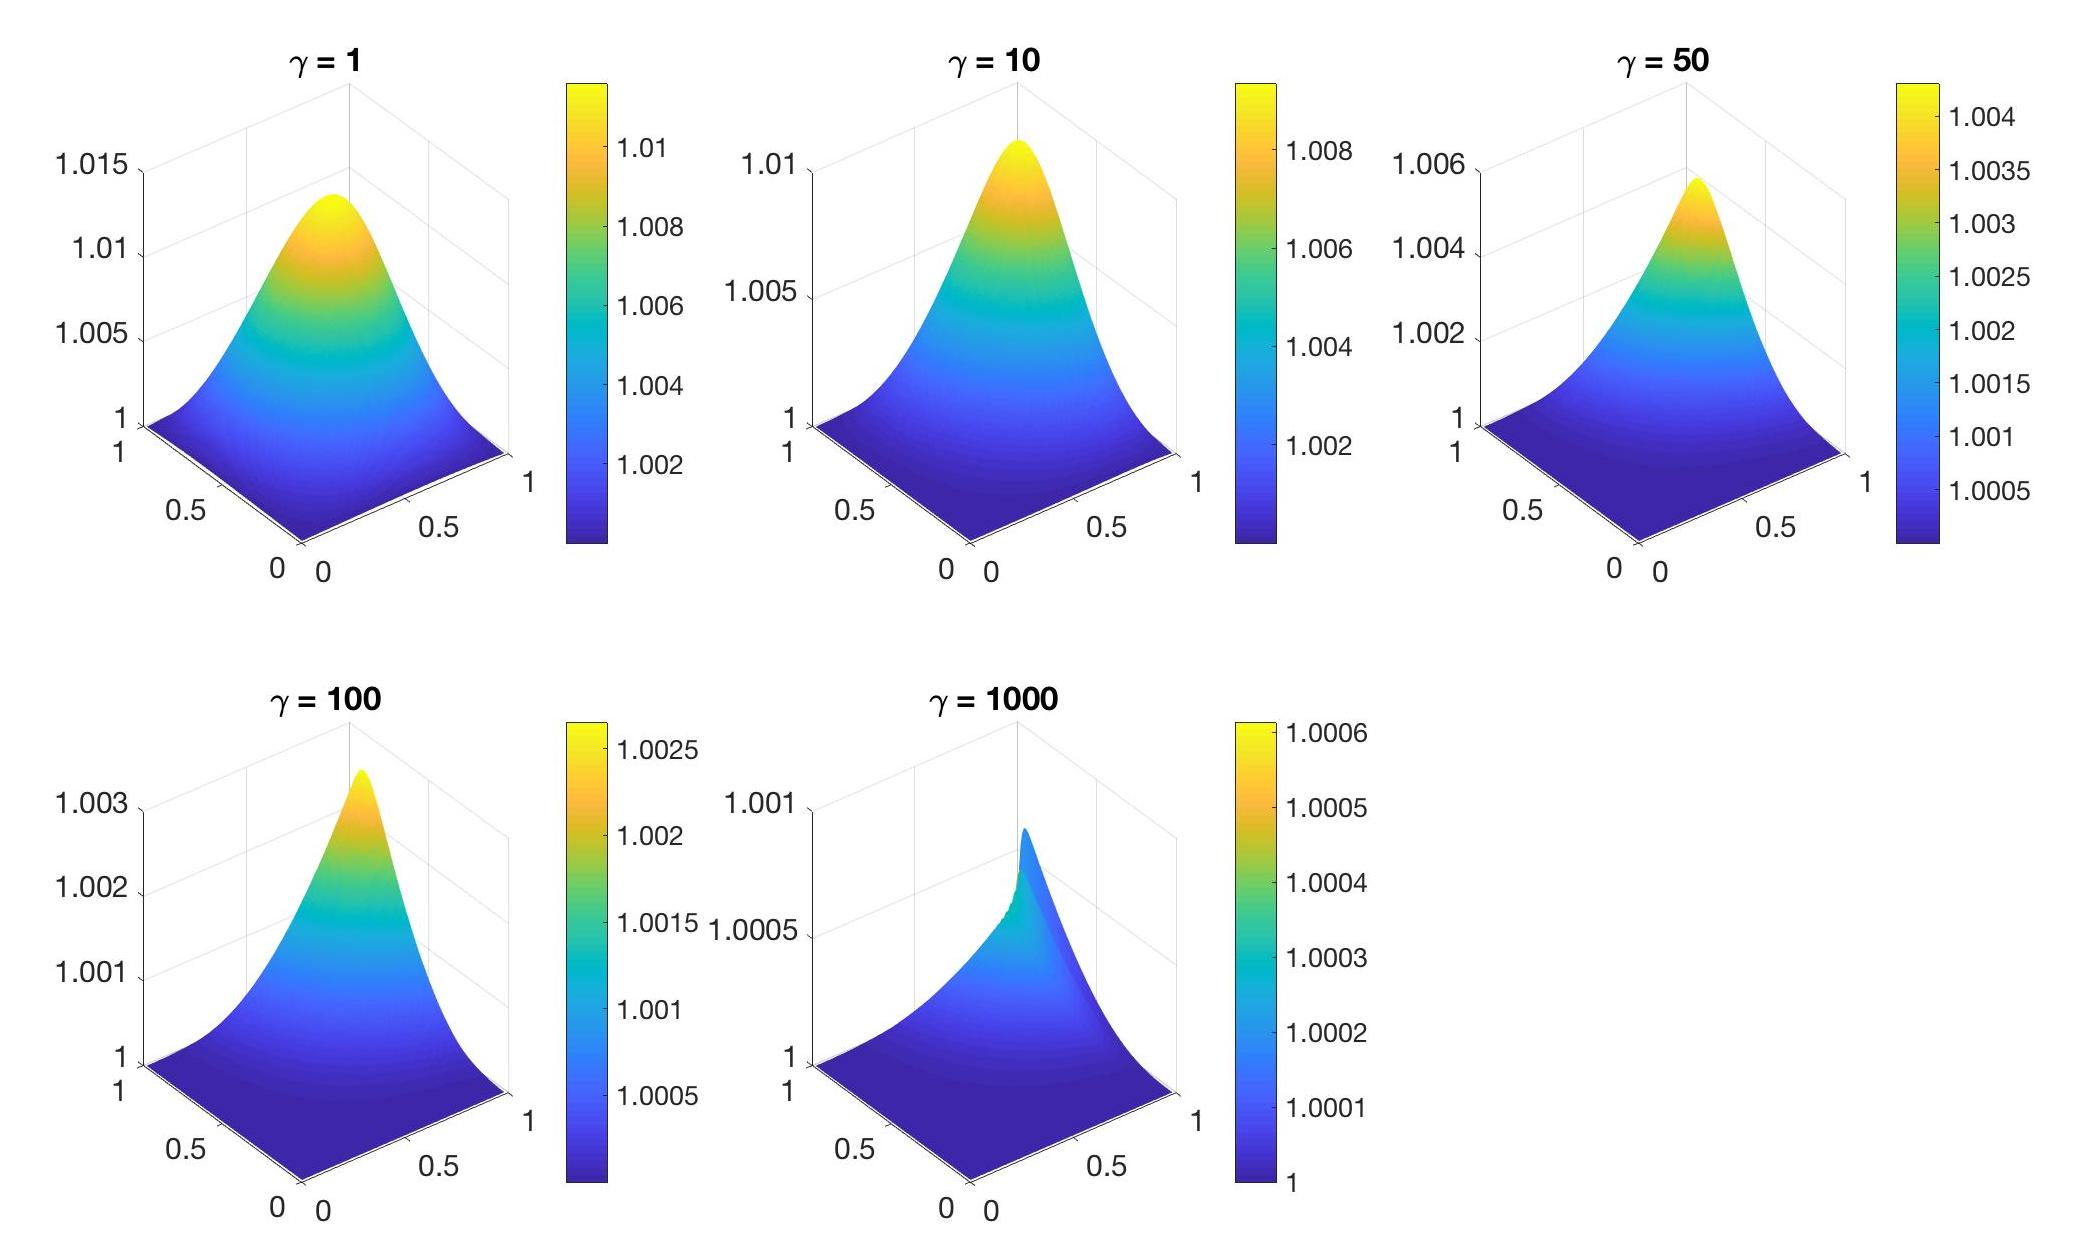
\includegraphics[scale=.22]{Problem1_graphs.jpg}
\caption{Surface Plots of Solution $u$, for each $\gamma$}
\end{figure}

\begin{figure}[H]
\center
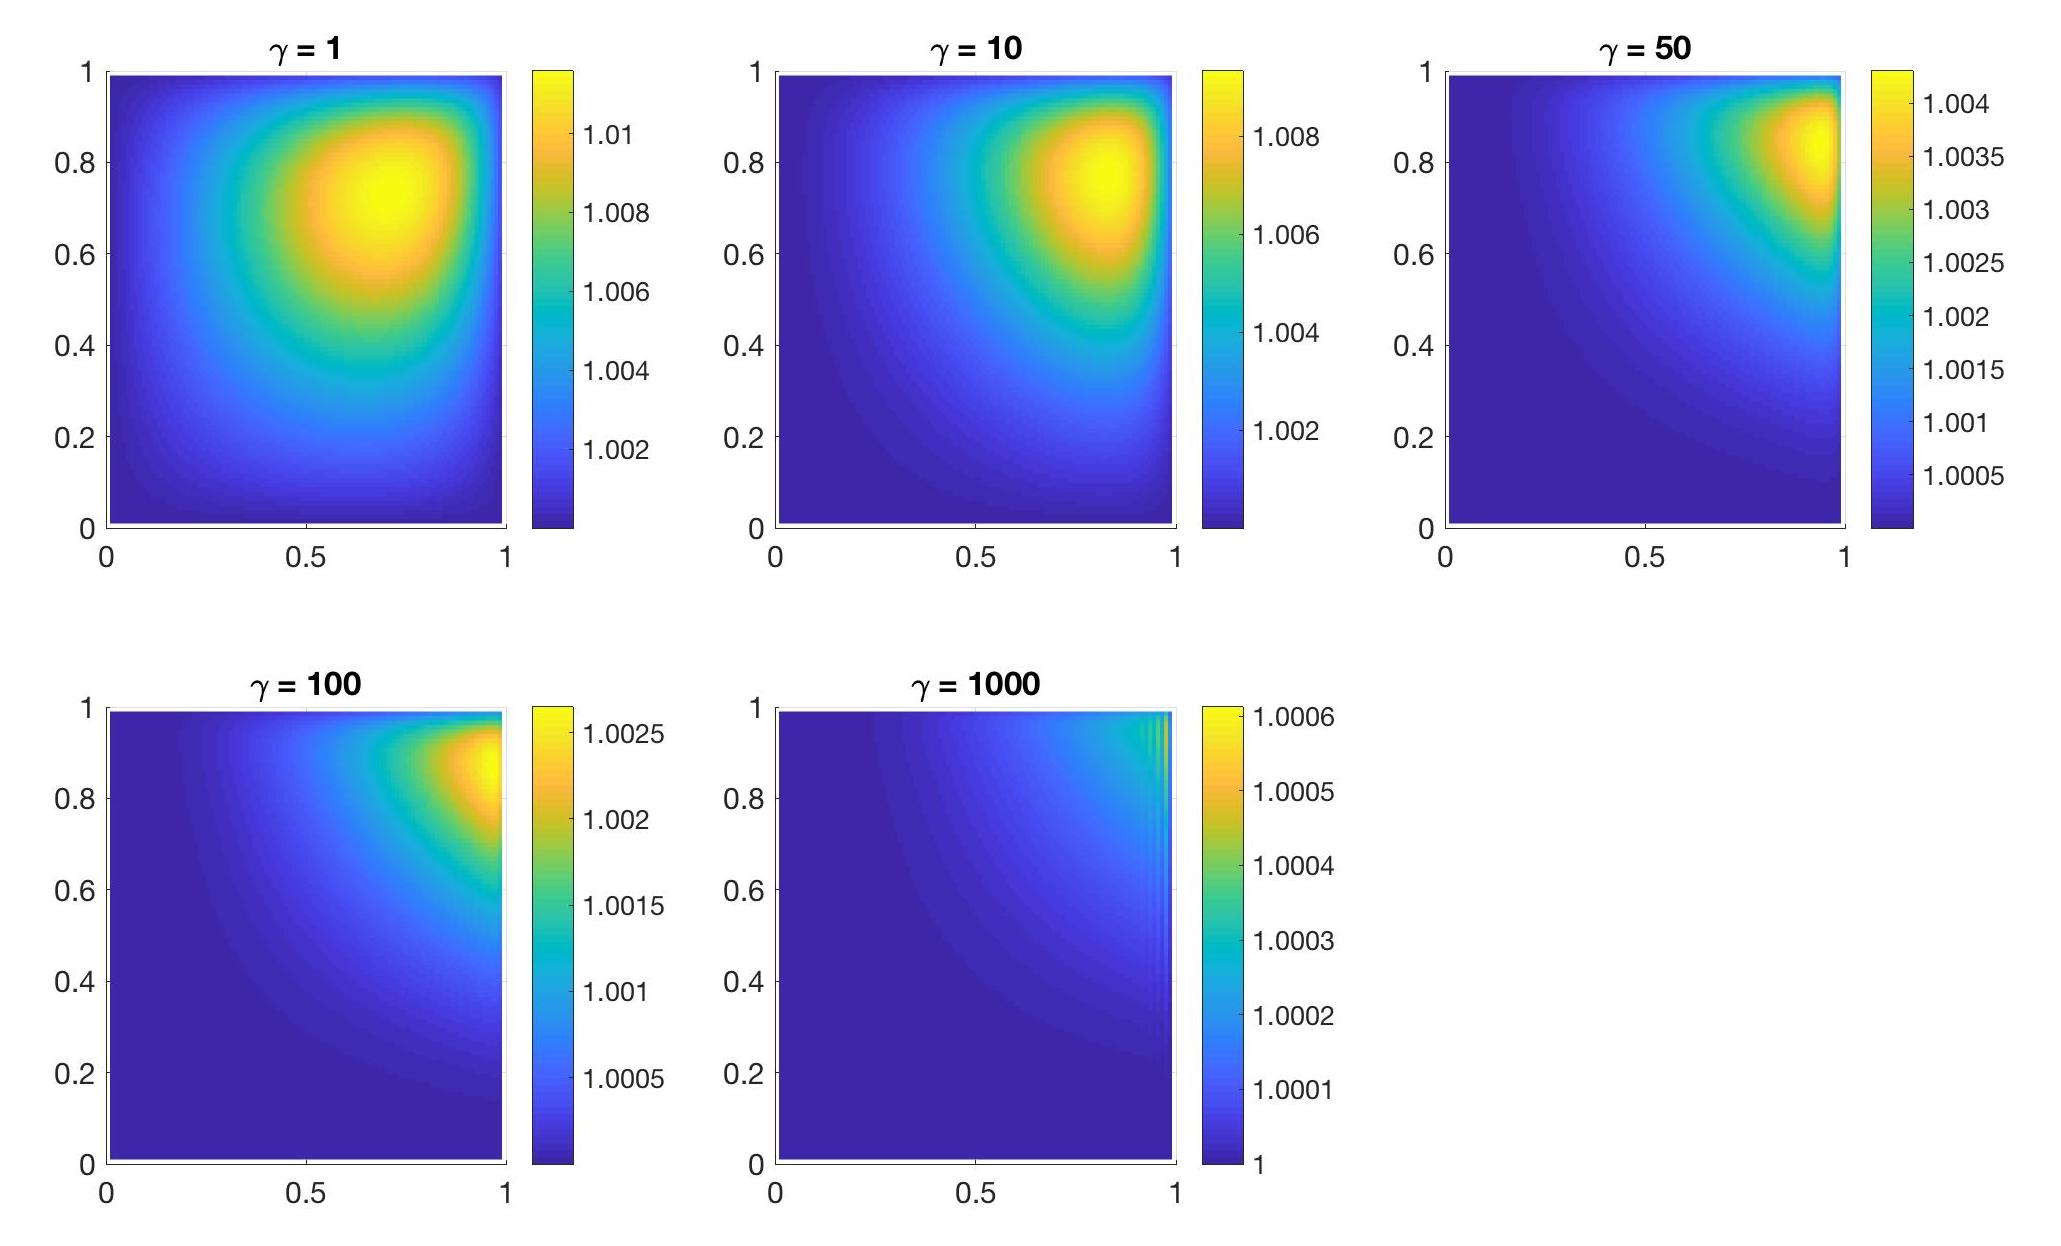
\includegraphics[scale=.22]{Problem1_heatmaps.jpg}
\caption{Heat Maps of Solution $u$, for each $\gamma$}
\end{figure}

\begin{figure}[H]
\center
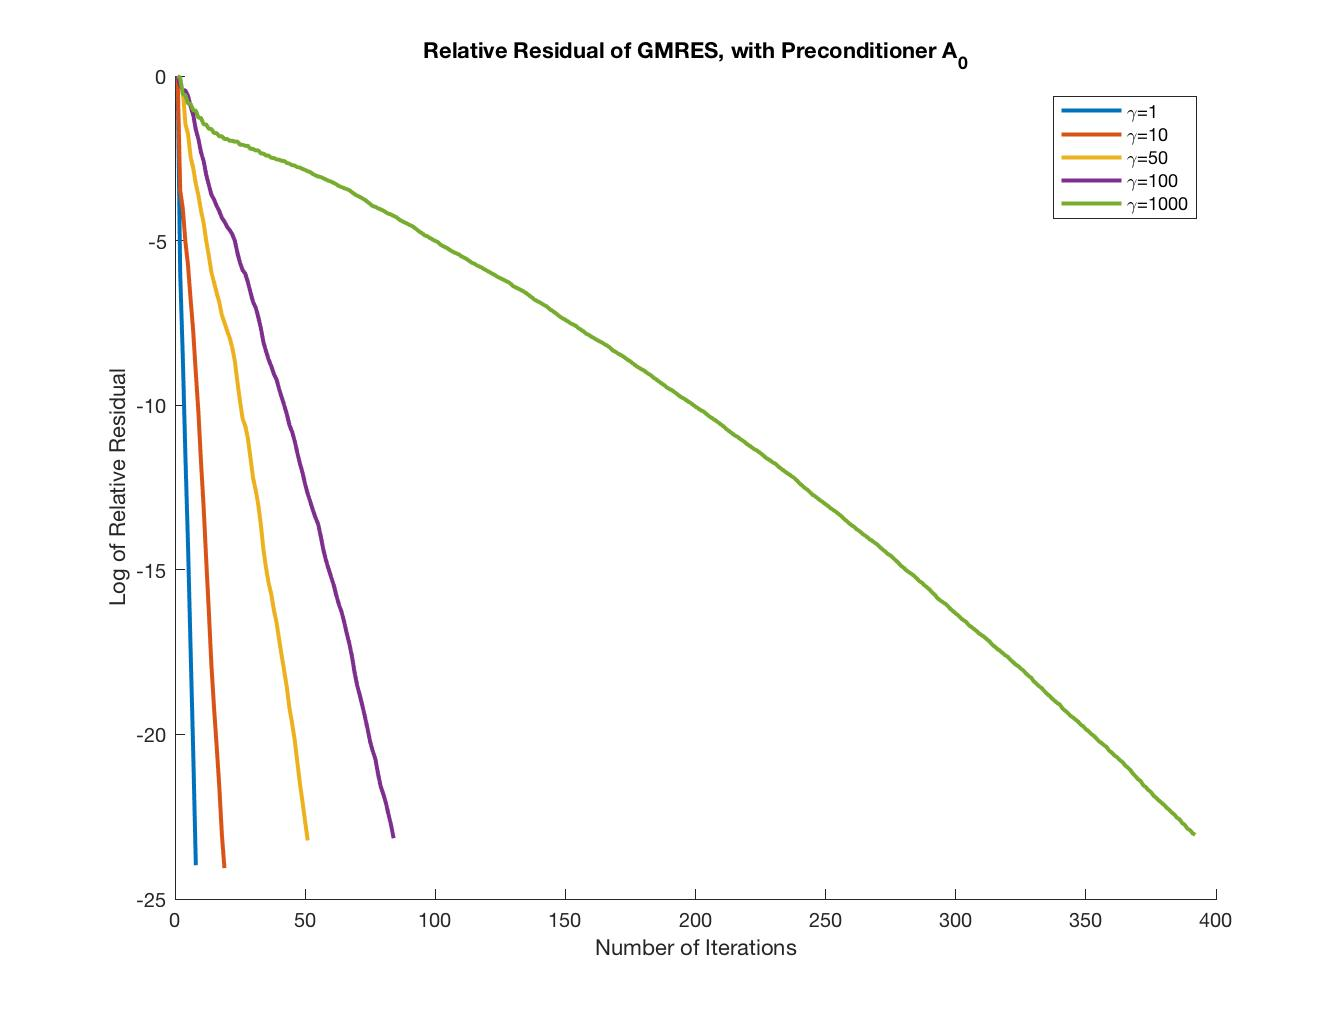
\includegraphics[scale=.33]{Problem1_relresGraph.jpg}
\caption{Plot of Log of Relative Residuals using GMRES for each $\gamma$}
\end{figure}
\noindent
As is shown in the above figure, as $gamma$ increases, the number of iterations also significantly increase.\qed\\


\newpage
\section{Problem 2} 
\begin{mybox}{Cerulean}{}
Let $A\in\R^{n\times n}$, $A \succ 0$, $b, x_0 \in \R^n$, and $r_0 := b- Ax_0$.  Let
$$x_k^{CG}, \text{ } k = 1, 2, \dots, d(A,r_0),$$
denote the iterates produced by the CG algorithm applied to $Ax=b$ with initial guess $x_0$.\\
Show that for every $k=1,2,\dots,d(A,r_0)$, $x_k^{CG}$ satisfies the following relation
$$x_k^{CG} = x_0 + V_kz_k, \text{ where } z_k :=\|r_0\|_2T_k^{-1}e_1^{(k)}.$$
Here, $e_1^{(k)}$ denotes the first unit vector of length $k$, $T_k$ is the tridiagonal matrix generated by $k$ steps of the Hermitian Lanczos process applied to $A$ and $r_0$, and $V_k$ denotes the $n\times k$ matrix that contains the corresponding first $k$ Lanczos vectors as columns.
\end{mybox}
\text{ }\\
\noindent
To show that $x_k^{CG} = x_0 + V_kz_k$ for every $k=1,2,\dots,d(A,r_0)$, $x_k^{CG}$, we want to minimize the error with respect to the A-norm, and show that $z_k =\|r_0\|_2T_k^{-1}e_1^{(k)}$.  Thus, it follows that:
\begin{align*}
E(z_k) &= \| x^* - x_k^{CG}\|_A \\
&= \| x^* - (x_0 + V_kz_k)\|_A \\
&= \big(x^* - (x_0 + V_kz_k)\big)^T A \big(x^* - (x_0 + V_kz_k)\big) 
\end{align*}
where $x^*$ denotes the actual solution.  Now, to find the minimum of $E(z_k)$, we need to find where $E'(z_k) = 0$.
\begin{align*}
E'(z_k) &= 2V_k^T\big(Ax^* - Ax_0 - AV_kz_k\big) \\
&= 2V_k^T\big(b - Ax_0 - AV_kz_k\big) \\
&= 2V_k^T\big(r_0 - AV_kz_k\big)
\end{align*}
\begin{align*}
E'(z_k) &= 0 \\
2V_k^T\big(r_0 - AV_kz_k\big) &= 0 \\
V_k^Tr_0 &= V_k^TAV_kz_k \\
V_k^T &= T_kz_k \\
T_kz_k &= V_k^T\big(v_1\|r_0\|_2\big) \\
T_kz_k &= e_1^{(k)}\|r_0\|_2 \\
z_k &= \|r_0\|_2T_k^{-1}e_1^{(k)}
\end{align*}
Thus, the CG algorithm applied to $Ax=b$ with initial guess $x_0$ satisfies $x_k^{CG} = x_0 + V_kz_k$, where $z_k :=\|r_0\|_2T_k^{-1}e_1^{(k)}$, for every $k=1,2,\dots,d(A,r_0)$, $x_k^{CG}$.\qed\\

\newpage
\section{Problem 3} 
\begin{mybox}{Cerulean}{}
Let $A\in \C^{n\times n}$ be a large sparse Hermitian matrix and $b\in \C^n$, $b\neq 0$.  Consider the vector-valued function $g: \C \to \C^n$ defined by 
$$g(\lambda) := e^{A\lambda}b \text{ for all } \lambda\in\C.$$
How can you use the Hermitian Lanczos process to generate approximations
$$g_k(\lambda) \approx g(\lambda), \text{ } k=1,2,\dots, d(A,b),$$
that for each $\lambda \in\C$ can be evaluated by computing the value of only a $k\times k$ matrix function (instead of an $n\times n$ matrix function for $g(\lambda)$)?
\end{mybox}
\text{ }\\

\noindent
Let $\overline{A} = A\lambda$.  Then,
\begin{align*}
g(\lambda) &= e^{A\lambda}b \\
&= e^{\overline{A}}b,
\end{align*}
where
$$e^{\overline{A}} = \sum\limits_{j=0}^\infty \frac{1}{j!}\overline{A}^j.$$
Now, we pick $r\in\C^n$, $r\neq 0$, and run Arnoldi for $k$ steps and get $H_k$ and $V_k$ such that $H_k = V_k^H\overline{A}V_k = V_k^H\lambda A V_k$.  Then,
\begin{align*}
\overline{A} &\approx V_kH_kV_k^H \\
\overline{A}^2 &\approx V_kH_kV_k^HV_kH_kV_K^H \\
&\approx V_kH_k^2V_k^H \\
&\vdots \\
\overline{A}^j &\approx V_kH_k^jV_k^H
\end{align*}
for $j=0,1,\dots $.  Then, we get:
\begin{align*}
e^{\overline{A}} &\approx \sum\limits_{j=0}^\infty \frac{1}{j!}V_kH_k^jV_k^H \\
&= V_k\bigg(\sum\limits_{j=0}^\infty \frac{1}{j!}H_k^j\bigg)V_k^H \\
&= V_k e^{H_k}V_k^H
\end{align*}
for $k=1,2,\dots, d(A,b)$.  Then, we get
$$g_k(\lambda) \approx \big(V_k e^{H_k}V_k^H\big)b.$$
Now, if we choose $r = b$, then $v_1 = \frac{b}{\|b\|_2}$.  It follows that $v_j^Hb = v_j^Hv_1\|b\|_2 = 0$ for $j > 1$.  Thus,
\begin{align*}
g_k(\lambda) &\approx \big(V_k e^{H_k}V_k^H\big)b \\
&= \big(V_k e^{H_k}\big)V_k^Hb \\
&= \big(V_k e^{H_k}\big)\|b\|_2 e_1 \\
&= \|b\|_2\big(V_k e^{H_k}\big)e_1
\end{align*}
Thus, using the Hermitian Lanczos process we get the approximation:
$$g_k(\lambda) \approx \|b\|_2\big(V_k e^{H_k}\big)e_1,$$
which can be evaluated by computing only a $k\times k$ matrix function, $e^{H_k}$, instead of an $n\times n$ matrix function.\qed\\


\newpage
\section{Problem 4} 
\begin{mybox}{Cerulean}{}
Write a Matlab program that implements the Arnolid process for matrices $A\in\C^{n\times n}$ and starting vectors $r\in\C^n$, $r\neq 0$, as presented in class.  Use an input parameter $k_{max}$ to limit the maximum number of Arnoldi steps.  The output of your program should be ther upper-Hessenber matrix $\tilde{H}_k \in\C^{(k+1)\times k}$ and the matrix $V_{k+1}\in\C^{n\times(k+1)}$ with the first $k+1$ Arnoldi vectors, where $k$ is the iteration index at termination of your algorithm.\\
Employ your implementation of the Arnoldi process to compute approximate eigenpairs of the matrix $A = A(\gamma)$ from (3) of Problem 1, where again $m=100$.  For each of the 5 values of $\gamma$ in (4), use the starting vector $r$ provided in the Matlab file $\text{"HW5\_P4.mat"}$ and $k_{max} = 300$.  Employ Matlab's "eig" function to compute the eigenpairs $(\tilde{\lambda}_j,z_j)$, $j=1,2,\dots,k$, of $H_k$.  Use the formula derived in class, to compute the residual norm
$$\rho_j = \|A\tilde{x}_j = \tilde{\lambda}_j\tilde{x}_j\|_2$$
of the approximate eigenpairs $(\tilde{\lambda}_j,\tilde{x}_j)$, $j=1,2,\dots,k$, of $A$, without computing the approximate eigenvectors $\tilde{x}_j$.\\
For each of your 5 runs (one for each value of $\gamma$), print out
$$\min_{1\leq j \leq k} \rho_j \text{ and } \max_{1\leq j \leq k} \rho_j,$$
together with all the approximate eigenvalues $\tilde{\lambda}_j$ for which the minimum and maximum is attained, and submit a plot that shows all $k$ approximate eigenvalues of $A$.
\end{mybox}

\lstset{language=matlab,frame=single}
\begin{lstlisting}[caption=Matlab Code to Compute Approximate Eigenpairs using the Arnoldi Process]
function [H,V] = Arnoldi(kmax)

format long e

load('HW5_P4.mat') % uploads r vector

m = 100;
n = m^2;
k = kmax;
beta = norm(r);
V = zeros(n,k+1);
V(:,1) = r/beta;
H_tilde = zeros(k+1,k);
gammaVec = [1, 10, 50, 100, 1000];

for g = 1:length(gammaVec)
    for j = 1:k
        q = ApMult(V(:,j),gammaVec(g),m);

        for i = 1:j
            H_tilde(i,j) = V(:,i)'*q;
            q = q - H_tilde(i,j)*V(:,i);
        end

        H_tilde(j+1,j) = norm(q);

        if (H_tilde(j+1,j) == 0)
            k = j;
            break
        end

        V(:,j+1) = q/H_tilde(j+1,j);

    end

    % compute eigenpairs of Hk
    Hk = H_tilde(1:k,1:k);
    [z,lambdaMat] = eig(Hk);
    lambda_approx = diag(lambdaMat);

    % compute the residual norm of the approximate eigenpairs without 
    % computing the approximate eigenvectors
    j = [1:1:k];
    rho = H_tilde(k+1,k).*abs(z(k,j));
    rho = rho';
    gammaVec(g)
    error = (norm(rho))

    min_rho_val = min(rho)
    max_rho_val = max(rho)
    [row_min] = find(rho == min_rho_val);
    [row_max] = find(rho == max_rho_val);
    
    row_min
    min_lams = lambda_approx(row_min)
    row_max
    max_lams = lambda_approx(row_max)

    figure(1)
    hold on
    subplot(2,3,g)
    plot(1:k,lambda_approx)
    xlabel('k')
    ylabel("Approximate Eigenvalue, \lambda_k, of A")
    title(strcat("\gamma = ", num2str(gammaVec(g))))
    
    figure(2)
    subplot(2,3,g)
    plot(real(lambda_approx),imag(lambda_approx),'x')
    xlabel("Real Part of \lambda_k")
    ylabel("Imaginary Part of \lambda_k")
    title(strcat("\gamma = ", num2str(gammaVec(g))))
end
end
\end{lstlisting}


\begin{table}[H]
\centering
\renewcommand{\arraystretch}{1.5}
%\begin{small}
\begin{tabular}{| c || c | c |}
\hline
& $\min \rho_j$ & $\max \rho_j$ \\
\hline
\hline
$\gamma = 1$ & 0  &  1.401291804925245e-01 \\
$\gamma = 10$ & 0  &  8.580633964789891e-03 \\
$\gamma = 50$ & 0  &  4.159214891729932e-02 \\
$\gamma = 100$ & 0 & 7.755234722789697e-02  \\
$\gamma = 1000$ & 0  & 8.129363507023497e-01  \\
\hline
\end{tabular}
%\end{small}
\caption{Minimum and Maximum $\rho$ Values for each $\gamma$}
\end{table} 


\begin{table}[H]
\centering
\renewcommand{\arraystretch}{1.5}
\begin{small}
\begin{tabular}{| c | c || c | c |}
\hline
$\gamma = 1$ &  \textbf{Minimum $\tilde{\lambda}_j$} &   &  \textbf{Maximum $\tilde{\lambda}_j$} \\
\hline 
\hline
$\tilde{\lambda}_1$ & 6.062023573145691e-16 + 0.000000000000000e+00i  & $\tilde{\lambda}_{300}$ &  4.187624012843567e-02 \\
$\tilde{\lambda}_2$ & 2.175909987645476e-16 + 0.000000000000000e+00i  &  &   \\
$\tilde{\lambda}_3$ & -2.860131570788593e-16 + 0.000000000000000e+00i  &  &   \\
$\tilde{\lambda}_4$ & -3.642886965850457e-16 + 0.000000000000000e+00i  &  &   \\
$\tilde{\lambda}_5$ & 1.000000000000001e+00 + 1.124896368980698e-01i  &  &   \\
$\tilde{\lambda}_6$ & 1.000000000000001e+00 - 1.124896368980698e-01i  &  &   \\
$\tilde{\lambda}_7$ & 6.145481823383067e-16 + 0.000000000000000e+00i  &  &   \\
$\tilde{\lambda}_8$ &  -4.763519902514354e-16 + 2.263097093527045e-16i  &  &   \\
$\tilde{\lambda}_9$ & -4.763519902514354e-16 - 2.263097093527045e-16i  &  &   \\
$\tilde{\lambda}_{10}$ & -1.440974982318229e-17 + 0.000000000000000e+00i  &  &   \\
\hline
\end{tabular}
\end{small}
\caption{Approximate Eigenvalues Corresponding to the Minimum and Maximum $\rho_j$ Values for $\gamma = 1$}
\end{table} 

\begin{table}[H]
\renewcommand{\arraystretch}{1.5}
\begin{small}
\hspace{-.85in}
\begin{tabular}{| c | c || c | c |}
\hline
$\gamma = 10$ &  \textbf{Minimum $\tilde{\lambda}_j$} &   &  \textbf{Maximum $\tilde{\lambda}_j$} \\
\hline 
\hline
$\tilde{\lambda}_1$ & 1.000000000000004e+00 + 1.124896368980693e+00i  & $\tilde{\lambda}_{291}$ & 9.999586452946625e-01 + 6.220077626936730e-02i  \\
$\tilde{\lambda}_2$ & 1.000000000000004e+00 - 1.124896368980693e+00i  & $\tilde{\lambda}_{292}$ &  9.999586452946625e-01 - 6.220077626936730e-02i \\
\hline
\end{tabular}
\end{small}
\caption{Approximate Eigenvalues Corresponding to the Minimum and Maximum $\rho_j$ Values for $\gamma = 10$}
\end{table} 

\begin{table}[H]
\renewcommand{\arraystretch}{1.5}
\begin{small}
\hspace{-.9in}
\begin{tabular}{| c | c || c | c |}
\hline
$\gamma = 50$ &  \textbf{Minimum $\tilde{\lambda}_j$} &   &  \textbf{Maximum $\tilde{\lambda}_j$} \\
\hline 
\hline
$\tilde{\lambda}_1$ & 9.999999999999996e-01 + 5.624481844903448e+00i  & $\tilde{\lambda}_{265}$ & 1.000307573463644e+00 + 3.092463650198238e-01i  \\
$\tilde{\lambda}_2$ & 9.999999999999996e-01 - 5.624481844903448e+00i  & $\tilde{\lambda}_{266}$ &  1.000307573463644e+00 - 3.092463650198238e-01i \\
$\tilde{\lambda}_3$ & 1.000000000000002e+00 + 3.556289316821879e+00i  &  &   \\
$\tilde{\lambda}_4$ &  1.000000000000002e+00 - 3.556289316821879e+00i &  &   \\
$\tilde{\lambda}_5$ & 1.000000000000002e+00 + 3.553704482968801e+00i  &  &   \\
$\tilde{\lambda}_6$ & 1.000000000000002e+00 - 3.553704482968801e+00i
  &  &   \\
\hline
\end{tabular}
\end{small}
\caption{Approximate Eigenvalues Corresponding to the Minimum and Maximum $\rho_j$ Values for $\gamma = 50$}
\end{table} 

\begin{table}[H]
\renewcommand{\arraystretch}{1.5}
\begin{small}
\hspace{-.95in}
\begin{tabular}{| c | c || c | c |}
\hline
$\gamma = 100$ &  \textbf{Minimum $\tilde{\lambda}_j$} &   &  \textbf{Maximum $\tilde{\lambda}_j$} \\
\hline 
\hline
$\tilde{\lambda}_1$ & 9.999999999999959e-01 + 1.124896368980693e+01i  & $\tilde{\lambda}_{219}$ & 1.000575881075355e+00 + 2.346008072192732e-02i  \\
$\tilde{\lambda}_2$ & 9.999999999999959e-01 - 1.124896368980693e+01i  & $\tilde{\lambda}_{220}$ &  1.000575881075355e+00 - 2.346008072192732e-02i \\
$\tilde{\lambda}_3$ & 9.999999999999971e-01 + 7.112578633643746e+00i  &  &   \\
$\tilde{\lambda}_4$ & 9.999999999999971e-01 - 7.112578633643746e+00i  &  &   \\
$\tilde{\lambda}_5$ & 1.000000000000004e+00 + 7.107408965937610e+00i  &  &   \\
$\tilde{\lambda}_6$ & 1.000000000000004e+00 - 7.107408965937610e+00i  &  &   \\
\hline
\end{tabular}
\end{small}
\caption{Approximate Eigenvalues Corresponding to the Minimum and Maximum $\rho_j$ Values for $\gamma = 100$}
\end{table} 

\begin{table}[H]
\renewcommand{\arraystretch}{1.5}
\begin{small}
\hspace{-.99in}
\begin{tabular}{| c | c || c | c |}
\hline
$\gamma = 1000$ &  \textbf{Minimum $\tilde{\lambda}_j$} &   &  \textbf{Maximum $\tilde{\lambda}_j$} \\
\hline 
\hline
$\tilde{\lambda}_1$ & 9.999999999999929e-01 + 1.124896368980693e+02i  & $\tilde{\lambda}_{287}$ & 9.751427114306593e-01 + 7.465537420048598e+00i  \\
$\tilde{\lambda}_2$ & 9.999999999999929e-01 - 1.124896368980693e+02i  & $\tilde{\lambda}_{288}$ &  9.751427114306593e-01 - 7.465537420048598e+00i \\
$\tilde{\lambda}_3$ & 9.999999999999876e-01 + 7.112578633643767e+01i  &  &   \\
$\tilde{\lambda}_4$ & 9.999999999999876e-01 - 7.112578633643767e+01i  &  &   \\
$\tilde{\lambda}_4$ & 1.000000000000022e+00 + 7.107408965937628e+01i  &  &   \\
$\tilde{\lambda}_6$ &  1.000000000000022e+00 - 7.107408965937628e+01i
 &  &   \\
\hline
\end{tabular}
\end{small}
\caption{Approximate Eigenvalues Corresponding to the Minimum and Maximum $\rho_j$ Values for $\gamma = 1000$}
\end{table} 

\begin{figure}[H]
%\center
\hspace{-.65in}
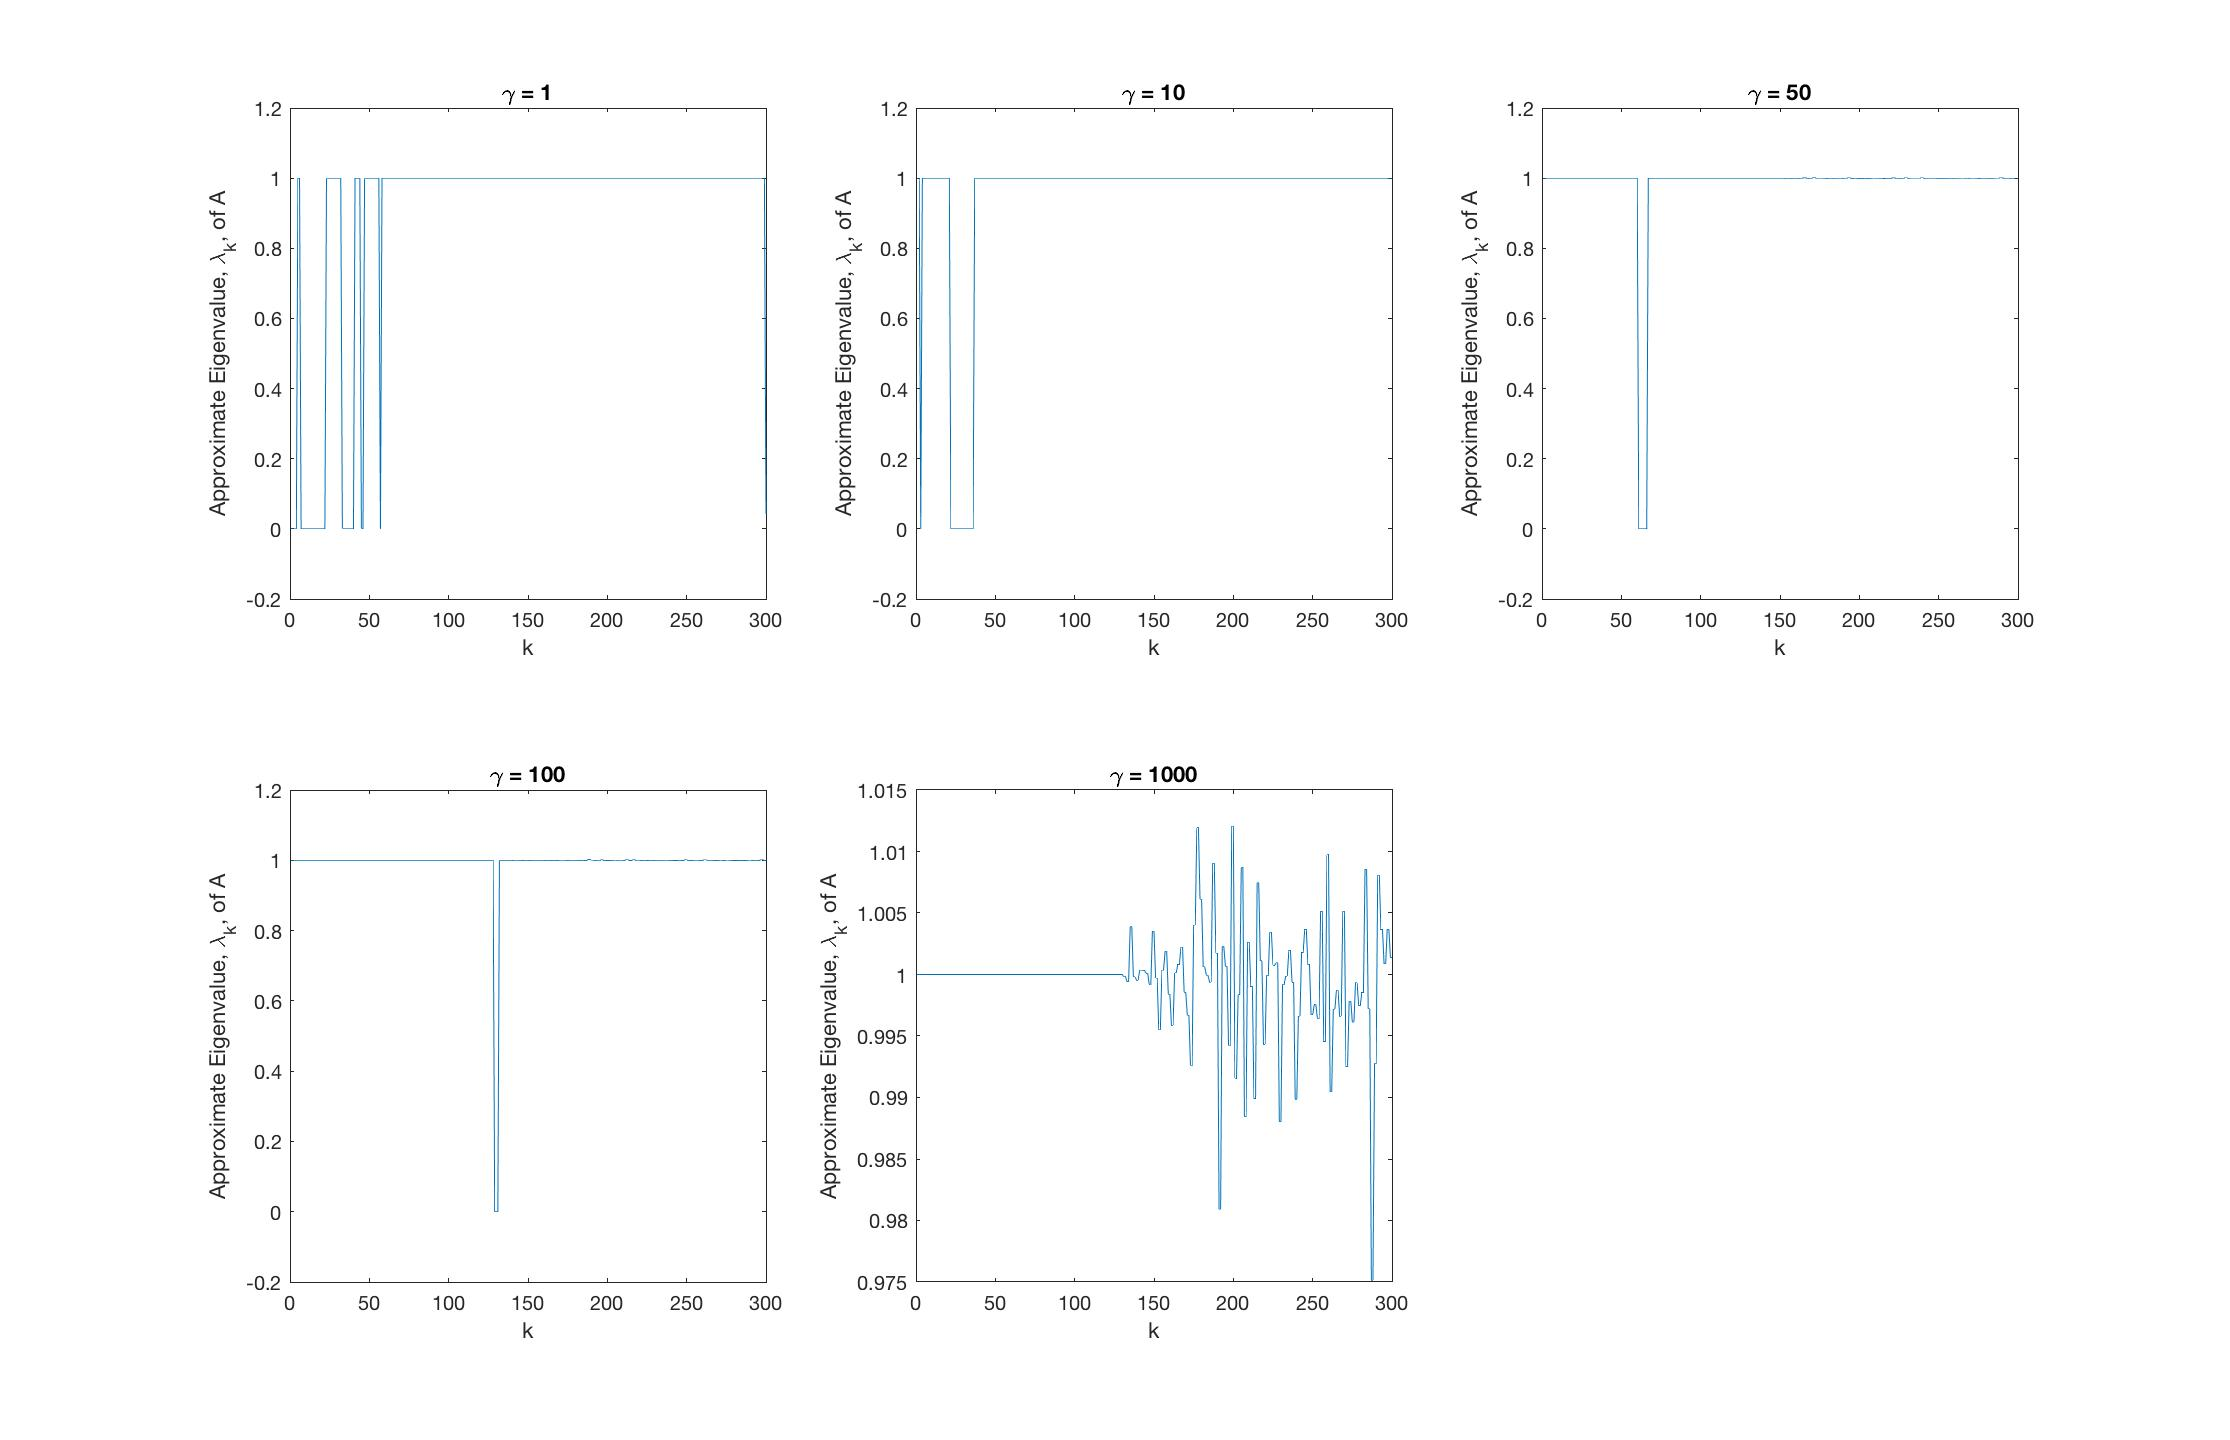
\includegraphics[scale=.25]{Problem4_graphs1.jpg}
\caption{Plots of Approximate Eigenvalues $\tilde{\lambda}_k$ vs. $k$ for each $\gamma$}
\end{figure}

\begin{figure}[H]
%\center
\hspace{-.65in}
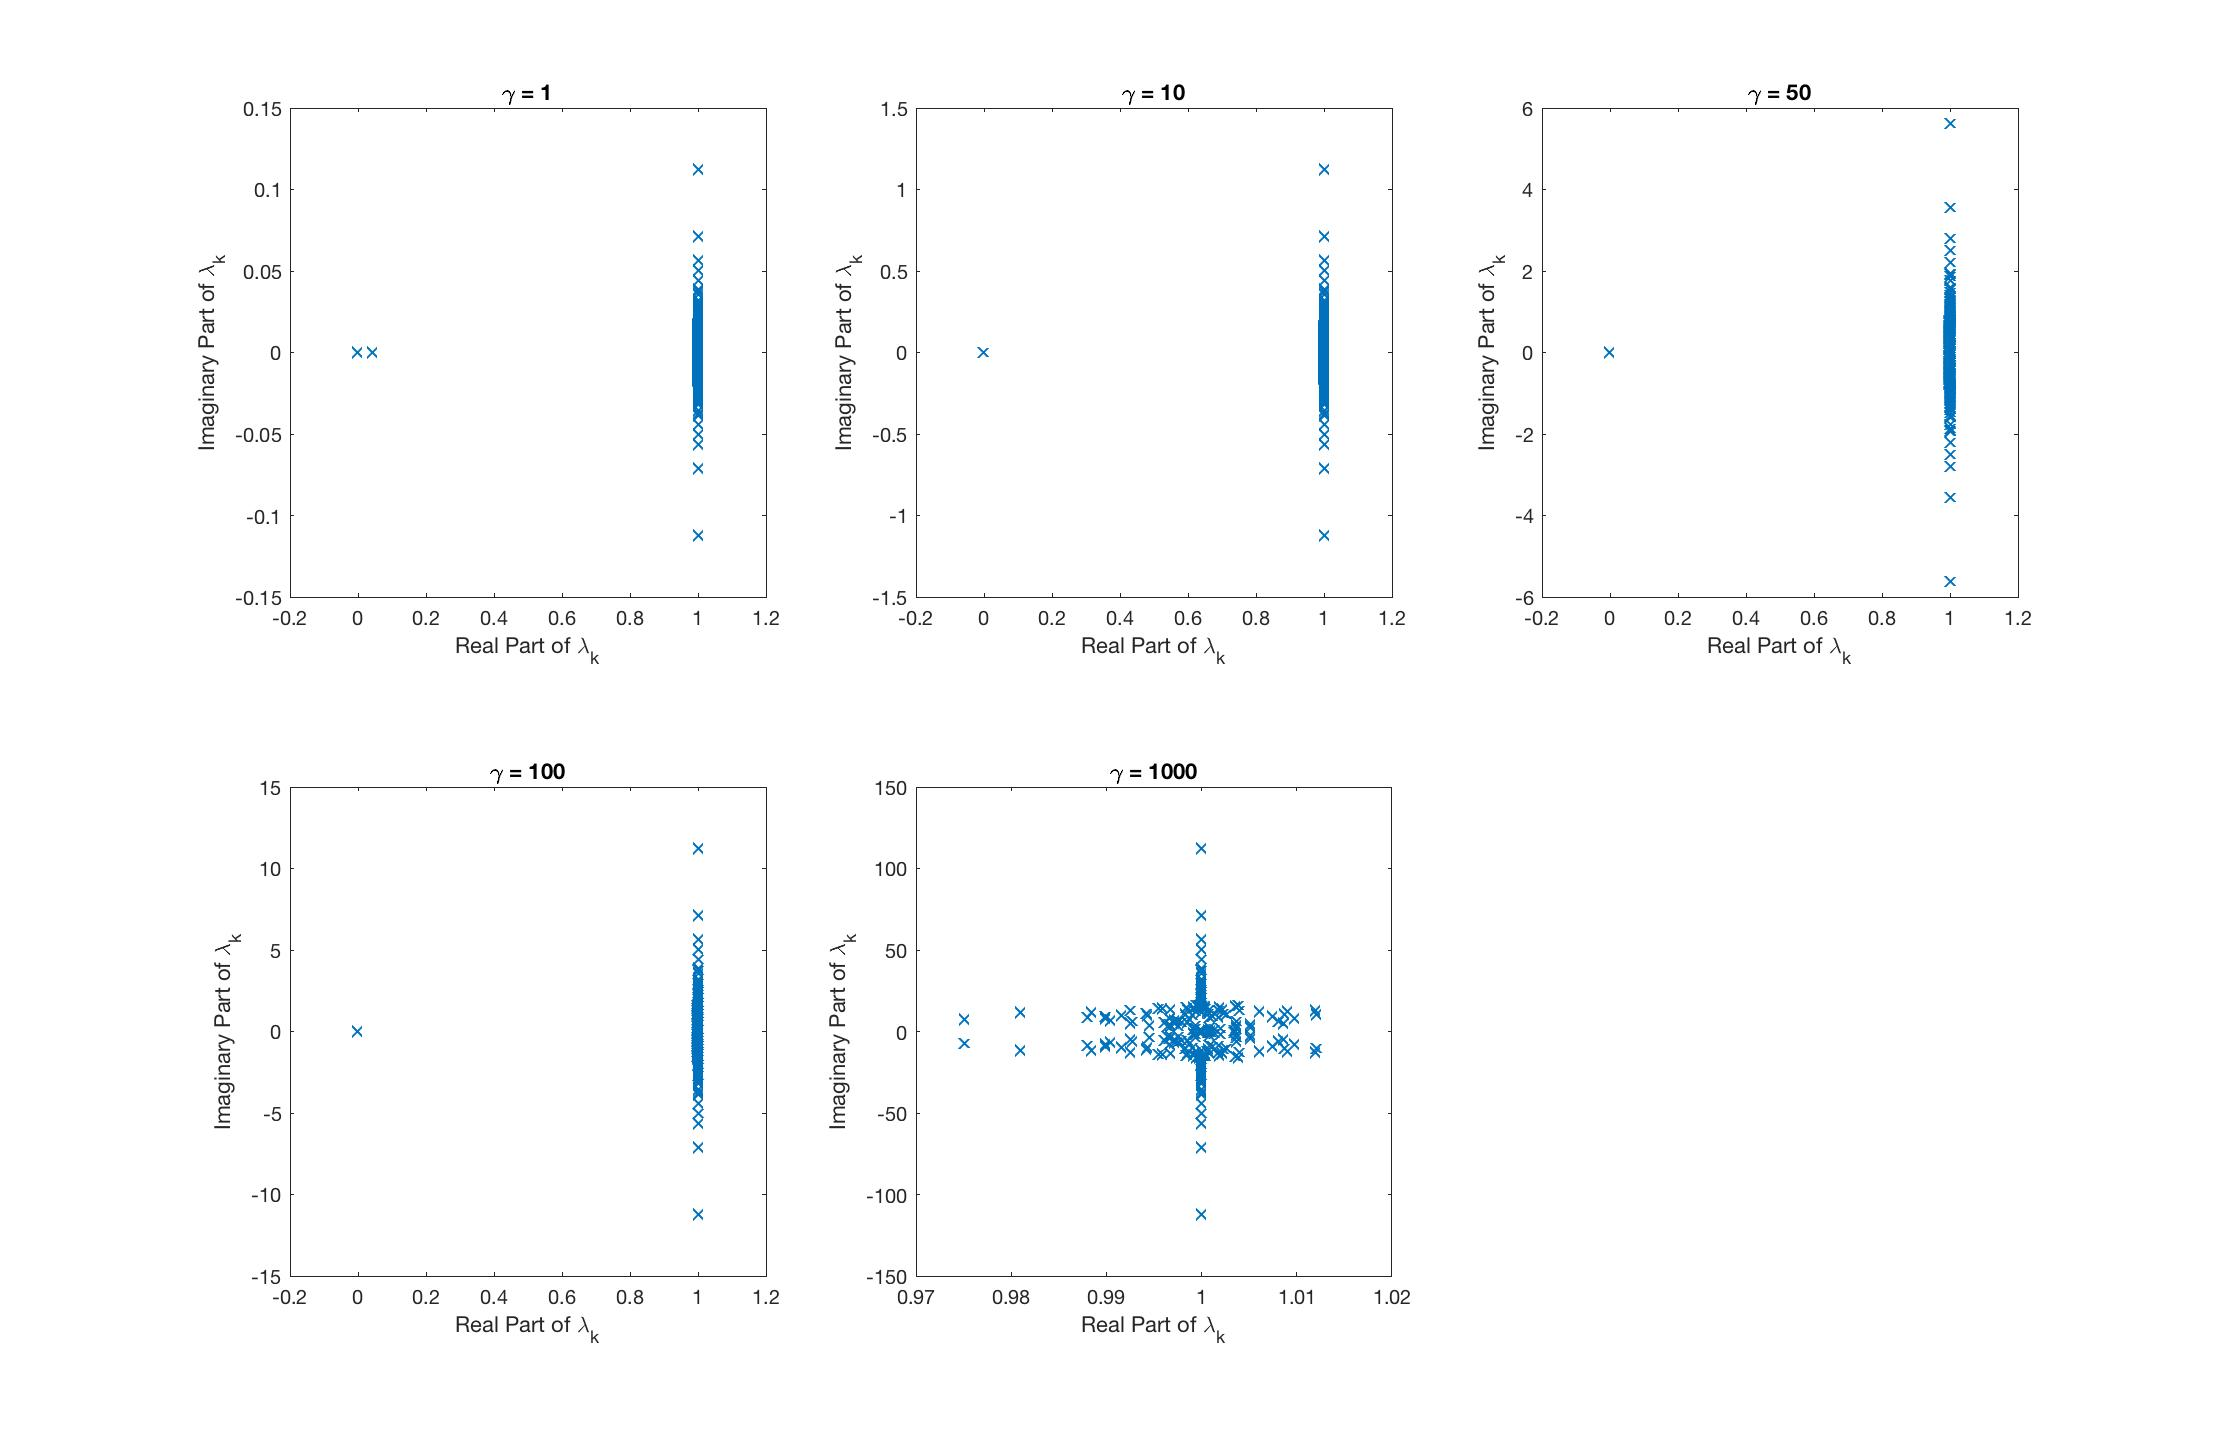
\includegraphics[scale=.25]{Problem4_graphs2.jpg}
\caption{Plots of Real vs. Imaginary Parts of Approximate Eigenvalues $\tilde{\lambda}_k$ for each $\gamma$}
\end{figure}
\qed\\



\newpage
\section{Problem 5} 
\begin{mybox}{Cerulean}{}
Write a Matlab program that implements the Hermitian Lanczos process for matrices $A = A^H \in\C^{n\times n}$ and starting vectors $r \in\C^n$, $r \neq 0$, as presented in class.  Use an input parameter $k_{max}$ to limit the maximum number of Lanczos steps.  Your program should only store the last two Lanczos vectors, $v_k$ and $v_{k-1}$, so that you can run the program for any number of steps.  The output of your routine should be the tridiagonal matrix $T_k \in \R^{k\times k}$, where $k$ is the iteration index at termination of your algorithm.\\
To test your program, use $n\times n$ matrices $A$ generated by
$$\text{A = make\_3d\_lapacian(m)}.$$
Note that $n=m^3$ and that the exact eigenvalues $\lambda = \lambda_{i,j,\ell}$ of $A$ are given by
$$\lambda_{i,j,\ell} = 2\bigg(3 - \cos\left(\frac{i\pi}{m+1}\right) - \cos\left(\frac{j\pi}{m+1}\right) - \cos\left(\frac{\ell\pi}{m+1}\right)\bigg), \text{ } i,j,\ell = 1,2,\dots,m.$$

\begin{itemize}

\item[(a)] Test your program on the $8\times 8$ matrix $A$ corresponding to $m=2$ and the starting vector $r$ provided in the Matlab file $\text{"HW5\_P5a.mat"}$.  Run the algorithm for $k_{max} = 4$ steps and commpute the eigenvalues of $T_4$ with Matlab's "eig" command.  Compare these eigenvalues with the exact eigenvalues of $A$.\\
\item[(b)] Employ your program to obtain approximate eigenvalues of the $328509\times 328509$ matrix $A$ corresponding to $m=69$, using the starting vector $r$ provided in the Matlab file $\text{"HW5\_P5b.mat"}$.  Compute the approximate eigenvalues obtained from the Lanczos matrices $T_k$ for
$$k = 250, 500, 1000, 2000.$$
For each of these values of $k$, print out the 10 smallest and the 10 largest eigenvalues of $T_k$ and compare them with the 10 smallest and the 10 largest exact eigenvalues of $A$.  What can you say about the quality of the approximate eigenvalues obtained from teh Lanczos process?\\
\end{itemize}
\end{mybox}

\newpage
\lstset{language=matlab,frame=single}
\begin{lstlisting}[caption= Matlab Code to Compute Approximate Eigenvalue using the Hermitian Lanczos Process]
function [Tk] = HermitianLanczos(kmax,m,fileNum)

format long e

if (fileNum == 1)
    load('HW5_P5a.mat')
elseif (fileNum == 2)
    load('HW5_P5b.mat')
end

A = make_3d_laplacian(m);
n = m^3;

tol = 1e-5;
alpha = zeros(kmax,1);
beta = zeros(kmax+1,1);

beta(1) = norm(r);
vk = r./beta(1);

for k=1:kmax
    
    q = A*vk;
    
    if (k > 1)
        q = q - beta(k)*v1;
    end
    
    alpha(k) = vk'*q;
    q = q - alpha(k)*vk;
    beta(k+1) = norm(q);
    
    if (beta(k+1) == 0)
        break
    end
    
    v1 = vk; %v1 = v_{k-1}
    vk=q./beta(k+1); %vk = v_{k+1}
end

% use alpha and beta vectors to construct Tk
Tk = diag(alpha,0) + diag(beta(2:kmax),-1) + diag(beta(2:kmax),1);

% now, use eig to compute the eigenvalues of Tk
lambda_approx = eig(Tk);
lambda_approx = uniquetol(lambda_approx,tol);

% compute exact eigenvalues to compare
i = [1:1:m]; j = [1:1:m]; l = [1:1:m];
[I,J,L] = meshgrid(i,j,l);
lambda_exact = 2*(3 - cos(I*pi/(m+1)) - cos(J*pi/(m+1)) - cos(L*pi/(m+1)));

lambda_exactVec = reshape(lambda_exact,[n,1]);
lambda_exactVec = uniquetol(lambda_exactVec,tol);

% for big case, find 10 smallest and 10 largest approximate and exact eigenvalues
if (fileNum == 2)
    lambda_approx = sort(lambda_approx);
    l1 = length(lambda_approx);
    lambda_exactVec = sort(lambda_exactVec);
    l2 = length(lambda_exactVec);
    
    smallest_approx = lambda_approx(1:10)
    smallest_exact = lambda_exactVec(1:10)
    
    biggest_approx = lambda_approx(end-9:end)
    biggest_exact = lambda_exactVec(end-9:end)
end
end
\end{lstlisting}

\begin{itemize}
\item[(a)] \text{ }\\

\begin{table}[H]
\centering
\renewcommand{\arraystretch}{1.5}
%\begin{small}
\begin{tabular}{| c || c | c |}
\hline
 &  \textbf{Approximate Eigenvalues} & \textbf{Exact Eigenvalues}\\
\hline 
\hline
$\lambda_1$ & 3.000000000000000e+00  &  3 \\
$\lambda_2$ & 5.000000000000003e+00  &  5 \\
$\lambda_3$ & 6.999999999999999e+00  &  7 \\
$\lambda_4$ & 9.000000000000002e+00  &  9 \\
\hline
\end{tabular}
%\end{small}
\caption{Comparison of approximate eigenvalues computed using the Hermitian Lanczos process, and the exact eigenvalues}
\end{table} 
\qed\\

\item[(b)] As we can see in the below tables, the quality of the eigenvalues obtained from the Lanczos process are very close to the exact eigenvalues.  For the smallest 10 eigenvalues, the approximations get closer to the exact eigenvalues as we increase $k$.  For the largest 10 eigenvalues, the approximations are very very close to the exact eigenvalues for all $k$, but get even closer to the exact values as $k$ increases.  Note that duplicate eigenvalues were removed before finding the 10 smallest and largest approximate and exact eigenvalues.  Since we are working with approximations and looking at 15 decimal places, in addition to removing eigenvalues that were exactly identical, I also removed and eigenvalues that were within a tolerance of $10^{-5}$ of any other eigenvalue.\\

\begin{table}[H]
%\centering
\renewcommand{\arraystretch}{1.5}
\begin{small}
\hspace{-.9in}
\begin{tabular}{| c | c | c || c | c | c |}
\hline
$k = 250$ &  \textbf{Smallest Approx} & \textbf{Smallest Exact} &   & \textbf{Largest Approx} & \textbf{Largest Exact}\\
\hline 
\hline
$\lambda_1$  &  6.041600777348929e-03  & 6.041600752111798e-03  & $\lambda_{328500}$  & 1.193967841648353e+01  &  1.195779389827037e+01 \\
$\lambda_2$  & 1.207914596602798e-02  &  1.207914584426284e-02 & $\lambda_{328501}$  & 1.194813249018734e+01  &  1.196178518015437e+01 \\
$\lambda_3$  & 1.811677334763728e-02  &  1.811669093641388e-02 & $\lambda_{328502}$  & 1.195560060935483e+01  &  1.196383144336252e+01 \\
$\lambda_4$  & 2.213178125207190e-02  & 2.212821029887158e-02  & $\lambda_{328503}$  & 1.196317078231754e+01  &  1.196579669951683e+01 \\
$\lambda_5$  & 2.817776082327112e-02  & 2.415423602856515e-02  & $\lambda_{328504}$  & 1.197046186175222e+01  &  1.197183424460898e+01 \\
$\lambda_6$  & 3.430388477604603e-02  & 2.816575539102262e-02  & $\lambda_{328505}$  & 1.197301741988887e+01  &  1.197584576397144e+01 \\
$\lambda_7$  & 4.073916196053342e-02  & 3.420330048317366e-02  & $\lambda_{328506}$  & 1.197777726554531e+01  &  1.197787178970113e+01 \\
$\lambda_8$  & 4.844284495010276e-02  & 3.616855663748186e-02  & $\lambda_{328507}$  & 1.198186057903147e+01  &  1.198188330906359e+01 \\
$\lambda_9$  &  5.491496666673977e-02 & 3.821481984563135e-02  & $\lambda_{328508}$  & 1.198792085346275e+01  &  1.198792085415574e+01 \\
$\lambda_{10}$  & 6.427178030291032e-02  & 4.220610172963291e-02  & $\lambda_{328509}$  & 1.199395839789970e+01  &  1.199395839924789e+01 \\
\hline
\end{tabular}
\end{small}
\caption{Comparision of exact and approximate eigenvalues computed using the Hermitian Lanczos process for $k = 250$}
\end{table} 

\begin{table}[H]
%\centering
\renewcommand{\arraystretch}{1.5}
\begin{small}
\hspace{-.9in}
\begin{tabular}{| c | c | c || c | c | c |}
\hline
$k = 500$ &  \textbf{Smallest Approx} & \textbf{Smallest Exact} &   & \textbf{Largest Approx} & \textbf{Largest Exact}\\
\hline 
\hline
$\lambda_1$  & 6.041600752111682e-03  & 6.041600752111798e-03  & $\lambda_{328500}$  & 1.195779390071517e+01  &  1.195779389827037e+01 \\
$\lambda_2$  & 1.207914584426521e-02  &  1.207914584426284e-02 & $\lambda_{328501}$  & 1.196178518246027e+01  &  1.196178518015437e+01 \\
$\lambda_3$  & 1.811669093641410e-02  &  1.811669093641388e-02 & $\lambda_{328502}$  & 1.196383144337132e+01  &  1.196383144336252e+01 \\
$\lambda_4$  & 2.212821029887092e-02  & 2.212821029887158e-02  & $\lambda_{328503}$  & 1.196579669952040e+01  &  1.196579669951683e+01 \\
$\lambda_5$  & 2.415423602856659e-02  & 2.415423602856515e-02  & $\lambda_{328504}$  & 1.197183424460897e+01  &  1.197183424460898e+01 \\
$\lambda_6$  & 2.816575539102289e-02  & 2.816575539102262e-02  & $\lambda_{328505}$  & 1.197584576397144e+01  &  1.197584576397144e+01 \\
$\lambda_7$  & 3.420330048307895e-02  & 3.420330048317366e-02  & $\lambda_{328506}$  & 1.197787178970113e+01  &  1.197787178970113e+01 \\
$\lambda_8$  & 3.616855658492681e-02  & 3.616855663748186e-02  & $\lambda_{328507}$  & 1.198188330906359e+01  &  1.198188330906359e+01 \\
$\lambda_9$  & 3.821481941474132e-02  & 3.821481984563135e-02  & $\lambda_{328508}$  & 1.198792085415574e+01  &  1.198792085415574e+01 \\
$\lambda_{10}$  &  4.220609548937836e-02 & 4.220610172963291e-02  & $\lambda_{328509}$  & 1.199395839924789e+01  &  1.199395839924789e+01 \\
\hline
\end{tabular}
\end{small}
\caption{Comparision of exact and approximate eigenvalues computed using the Hermitian Lanczos process for $k = 500$}
\end{table} 

\begin{table}[H]
%\centering
\renewcommand{\arraystretch}{1.5}
\begin{small}
\hspace{-.95in}
\begin{tabular}{| c | c | c || c | c | c |}
\hline
$k = 1000$ &  \textbf{Smallest Approx} & \textbf{Smallest Exact} &   & \textbf{Largest Approx} & \textbf{Largest Exact}\\
\hline 
\hline
$\lambda_1$  & 6.041600752106037e-03  & 6.041600752111798e-03  & $\lambda_{328500}$  & 1.196012678999239e+01  &  1.195779389827037e+01 \\
$\lambda_2$  & 1.207914584426428e-02  &  1.207914584426284e-02 & $\lambda_{328501}$  & 1.196178518015437e+01  &  1.196178518015437e+01 \\
$\lambda_3$  &  1.811669093641226e-02 &  1.811669093641388e-02 & $\lambda_{328502}$  & 1.196382227737983e+01  &  1.196383144336252e+01 \\
$\lambda_4$  &  2.212821029887353e-02 & 2.212821029887158e-02  & $\lambda_{328503}$  & 1.196579304140577e+01  &  1.196579669951683e+01 \\
$\lambda_5$  & 2.415423602856661e-02  & 2.415423602856515e-02  & $\lambda_{328504}$  & 1.197183424460896e+01  &  1.197183424460898e+01 \\
$\lambda_6$  & 2.816575539102539e-02  & 2.816575539102262e-02  & $\lambda_{328505}$  & 1.197584576397142e+01  &  1.197584576397144e+01 \\
$\lambda_7$  & 3.420330048317605e-02  & 3.420330048317366e-02  & $\lambda_{328506}$  & 1.197787178970112e+01  &  1.197787178970113e+01 \\
$\lambda_8$  & 3.616855663748406e-02  & 3.616855663748186e-02  & $\lambda_{328507}$  & 1.198188330906359e+01  &  1.198188330906359e+01 \\
$\lambda_9$  & 3.821481984563355e-02  & 3.821481984563135e-02  & $\lambda_{328508}$  & 1.198791372575761e+01  &  1.198792085415574e+01 \\
$\lambda_{10}$  & 3.834496735573469e-02  & 4.220610172963291e-02  & $\lambda_{328509}$  & 1.199395839924786e+01  &  1.199395839924789e+01 \\
\hline
\end{tabular}
\end{small}
\caption{Comparision of exact and approximate eigenvalues computed using the Hermitian Lanczos process for $k = 1000$}
\end{table} 

\begin{table}[H]
%\centering
\renewcommand{\arraystretch}{1.5}
\begin{small}
\hspace{-.95in}
\begin{tabular}{| c | c | c || c | c | c |}
\hline
$k = 2000$ &  \textbf{Smallest Approx} & \textbf{Smallest Exact} &   & \textbf{Largest Approx} & \textbf{Largest Exact}\\
\hline 
\hline
$\lambda_1$  & 6.041600752108586e-03  & 6.041600752111798e-03  & $\lambda_{328500}$  & 1.195779389827035e+01  &  1.195779389827037e+01 \\
$\lambda_2$  & 1.207914584424712e-02  &  1.207914584426284e-02 & $\lambda_{328501}$  & 1.196178518015435e+01  &  1.196178518015437e+01 \\
$\lambda_3$  & 1.811669093641360e-02  &  1.811669093641388e-02 & $\lambda_{328502}$  & 1.196383144336250e+01  &  1.196383144336252e+01 \\
$\lambda_4$  & 1.896689878249162e-02  & 2.212821029887158e-02  & $\lambda_{328503}$  & 1.196579669951681e+01  &  1.196579669951683e+01 \\
$\lambda_5$  & 2.212821029886937e-02  & 2.415423602856515e-02  & $\lambda_{328504}$  &  1.197183424460495e+01 &  1.197183424460898e+01 \\
$\lambda_6$  & 2.415423602856083e-02  & 2.816575539102262e-02  & $\lambda_{328505}$  & 1.197584576397143e+01  &  1.197584576397144e+01 \\
$\lambda_7$  & 2.816575539102160e-02  & 3.420330048317366e-02  & $\lambda_{328506}$  & 1.197787178970111e+01  &  1.197787178970113e+01 \\
$\lambda_8$  & 3.420330048317428e-02  & 3.616855663748186e-02  & $\lambda_{328507}$  & 1.198184461037408e+01  &  1.198188330906359e+01 \\
$\lambda_9$  & 3.616855663747475e-02  & 3.821481984563135e-02  & $\lambda_{328508}$  & 1.198792085415573e+01  &  1.198792085415574e+01 \\
$\lambda_{10}$  & 3.821481984562576e-02  & 4.220610172963291e-02  & $\lambda_{328509}$  & 1.199395839911458e+01  &  1.199395839924789e+01 \\
\hline
\end{tabular}
\end{small}
\caption{Comparision of exact and approximate eigenvalues computed using the Hermitian Lanczos process for $k = 2000$}
\end{table} 
\qed\\
\end{itemize}





\end{document}

% insert Matlab code
\lstset{language=matlab,frame=single}
\begin{lstlisting}[caption=]

\end{lstlisting}

% import Matlab code directly
\lstinputlisting[style=Matlab-editor,basicstyle=\ttfamily\small]{codename.m}

% OR
\lstset{language=Matlab}
\lstinputlisting{HermitianLanczos.m}

% table template
\begin{table}[H]
\centering
\renewcommand{\arraystretch}{1.3}
\begin{small}
\begin{tabular}{| c | c |}
\hline
Result &  Value\\
\hline 

\hline
\end{tabular}
\end{small}
\caption{ }
\end{table} 

% insert jpeg
\begin{figure}[H]
\center
\includegraphics[scale=.39]{ .jpg}
\caption{ }
\end{figure}

% negative hspace - move figures/tables/etc over to the left
\hspace{-.5in}


% change text color
{\color{red} **colored text goes here}

% change the text size in math environment
\[\Scale[0.5]{y = \sin^2 x}\] 

% to put a colored box around something. can change color
\begin{mybox}{red}{Title}
Stuff in box
\end{mybox}

% put default colored box around something
\begin{tcolorbox}
Stuff in box
\end{tcolorbox}